\begin{enumerate}
\item We have decided that the event function isn't very valuable and so dropped it
from the requirements early in development.

\item We decided that having a website and active servers was important and so
added it early in development.

\item Our data flow has changed in that the client now updates the local
database without waiting for updates from the server to arrive. This was done so
that network latency didn't interfere with the user experiance. All actions are
still sent to oneself via the server, else multiple clients with the same key
wouldn't function.

\item The client-client protocol has been significantly expanded so that all
actions can be represented within it. This is so that if all one has is a
keypair to an account, that account may be fully recovered. An example of new
functionality in the protocol is that category creation and modification is
recorded on the server (via encrypted messages sent, and viewable, soley to
oneself). NB: The client-server protocol is wholly unaltered.

\item The datatypes in the database have changes due to the limitations of
SQLite.

\item The primary key in many database tables has changed from an arbitrary
value to a globally identifying cryptographic signature (from the message
establishing the relevent datum.)

\item The database doesn't make use of foreign keys because the combination of
network latency being potentially different for every message (due to Tor) and
asymmetric relationships and communication means that foreign keys will often
reference something that either doesn't exist yet or will never exist.
Furthermore in SQLite a foreign key can only reference one thing, and two of our
potential foreign keys don't always reference the same field. Therefore there is
only one possible foriegn key in our entire database: tCategoryMembers.catID
references tCategory.catID, and even that is tenuous at best as relies upon
undefined behaviour of the frontend. For these reasons we removed foreign keys
from the schema. The new database design is as follow:

\section{Logical table design version 2.0}

% tCategory
tCategory 
\begin{center}
    \begin{tabular}{ | l | l |}
    \hline
    catId & canSeePDATA \\ \hline
    \end{tabular}
\end{center}

%tCategoryMembers
tCategoryMembers
\begin{center}
    \begin{tabular}{ | l | l | l |}
    \hline
    pk & catID & userKey \\ \hline
    \end{tabular}
\end{center}

%tClaim
tClaim
\begin{center}
    \begin{tabular}{ | l | l | l |}
    \hline
    sig & name & claimTime \\ \hline
    \end{tabular}
\end{center}

%tRevocations
tRevocations
\begin{center}
    \begin{tabular}{ | l | l | l | l |}
    \hline
    key & sig & timeOfLeak & creationTime \\ \hline
    \end{tabular}
\end{center}

%tPostVisibleTo
tPostVisibleTo
\begin{center}
    \begin{tabular}{ | l | l | l |}
    \hline
    pk & postSig & key \\ \hline
    \end{tabular}
\end{center}

%tConvoKeys
tConvoKeys
\begin{center}
    \begin{tabular}{ | l | l | l |}
    \hline
    pk & convoID & key \\ \hline
    \end{tabular}
\end{center}

%tConvos
tConvos
\begin{center}
    \begin{tabular}{ | l | l |}
    \hline
    convoID & timeCreated \\ \hline
    \end{tabular}
\end{center}

%tUser
tUser
\begin{center}
    \begin{tabular}{ | l | l | l | l | l | l | l |}
    \hline
    key & username & knowName & email & name & gender & birthday \\ \hline
    \end{tabular}
\end{center}

%tComment
tComment
\begin{center}
    \begin{tabular}{ | l | l | l | l | l |}
    \hline
    sig & msgText & senderKey & parent & creationTime \\ \hline
    \end{tabular}
\end{center}

%tPost
tPost
\begin{center}
    \begin{tabular}{ | l | l | l | l | l |}
    \hline
    sig & msgText & time & recieverKey & sendersKey  \\ \hline
    \end{tabular}
\end{center}

%tConvoMessages
tConvoMessages
\begin{center}
    \begin{tabular}{ | l | l | l | l | l |}
    \hline
    pk & convoID & sendersKey & msgText & time\\ \hline
    \end{tabular}
\end{center}

%tEvent
tEvent
\begin{center}
    \begin{tabular}{ | l | l | l | l | l | l | l |}
    \hline
    sig & startTime & endTime & creatorKey & accepted & name & creationTime \\ \hline
    \end{tabular}
\end{center}

%tLike
tLike
\begin{center}
    \begin{tabular}{ | l | l | l |}
    \hline
    pk & likerKey & parent \\ \hline
    \end{tabular}
\end{center}

\subsection{Database design version 2.0}
\begin{landscape}
\begin{figure}[h]
    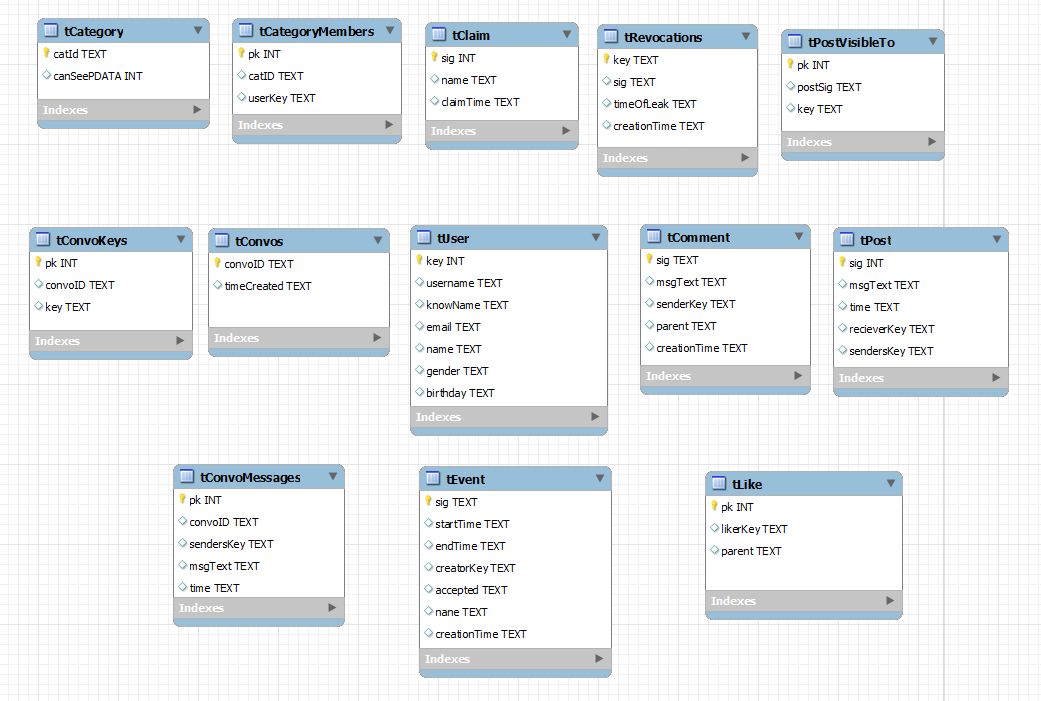
\includegraphics[width=1.4\textwidth]{images/design/db_shot.png}
    \caption{Database Entity Relationship diagram}
    \label{fig:db_er_diag}
\end{figure}
\end{landscape}



\item A number of accessors were added to the Message class for extracing
information from different types of messages.

\item The DBStrings class was added so as to keep SQL query strings seperate
from java code, and to localize them within one namespace. This class merely
contains a large number of static strings.

\item The Logger, Tokenizer,  MessageFactory, and F(ile)IO class were added as
helper classes. Tokenizer was created instead of using javas existing Tokenizer
class because we needed a tokenizer automatically convertable to javascript. A
factory class was required because the Message class cannot contain constructors
not automatically convertable to javascript.

\item The following data bearing classes were created to return structured data
to the HTML/JS frontend. They allow the more powerful java backend to extract
(and format) data from the database before returning a simple class containing
it.
\begin{enumerate}
\item Friend
\item CommentDetails
\item Conversation
\item PostDetails
\end{enumerate}

\item The Turtlenet, TurtlenetImpl, and TurtlenetAsync classes exist to provide
an asynchronous interface between the HTML/JS frontend and the Java backend.
\end{enumerate}

